\section{Development Environment and Tools}
\label{sec:env}

Table~\ref{tab:env} lists the environment in which the system was built and evaluated.

\begin{table}[htbp]
\centering
\caption{Development and evaluation environment}
\label{tab:env}
\small
\begin{tabularx}{\textwidth}{@{}P{4.0cm}L@{}}
\toprule
\textbf{Item} & \textbf{Version / detail} \\
\midrule
Runtime & Node.js (evaluation run on v24.20.0; the Netlify build configuration pins Node~20) \\
Package management & npm workspaces (\code{backend}, \code{frontend}); \code{concurrently} for running both in development \\
Backend & Express 4.19, Mongoose 8.5, Socket.IO 4.7, jsonwebtoken 9, bcryptjs 2.4, helmet 8.3, express-rate-limit 8.6, Nodemailer 10.1, PDFKit 0.15 (minimum versions of the caret ranges in \code{package.json}); \code{nodemon} for development \\
Frontend & React 19.1, React Router 7.8, Vite 7.1, Tailwind CSS 3.4, axios, socket.io-client 4.8, Leaflet 1.9 with leaflet-routing-machine, qrcode, @zxing/browser, @react-google-maps/api \\
Database & MongoDB (deployment via \code{MONGODB_URI}; evaluation with MongoDB~7.0.14 through mongodb-memory-server) \\
Quality tools & ESLint~9 (frontend), npm dependency audit \\
Evaluation machine & Windows~11 Pro, AMD Ryzen~5 5600X (6 cores, 12 threads), 15.9\,GB RAM \\
\bottomrule
\end{tabularx}
\end{table}

\section{Project Structure}
\label{sec:structure}

The repository is an npm workspace with two packages, \code{backend} and \code{frontend}, whose organisation is summarised in Table~\ref{tab:structure}.

\begin{table}[htbp]
\centering
\caption{Organisation of the repository}
\label{tab:structure}
\small
\begin{tabularx}{\textwidth}{@{}P{4.4cm}L@{}}
\toprule
\textbf{Folder} & \textbf{Contents and responsibility} \\
\midrule
\multicolumn{2}{@{}l}{\textbf{Backend package}} \\
\code{src/index.js}, \code{src/config} & Server start-up, middleware chain and database connection \\
\code{src/models} & Data models for users, parcels and sessions \\
\code{src/routes} & URL groups for authentication, parcels, users, assignments, analytics and geocoding \\
\code{src/controllers} & Business rules for authentication, parcels and analytics \\
\code{src/middleware} & Authentication and role guards, rate limits, input sanitising \\
\code{src/services} & Session handling, real-time socket handling and room-scoped messaging \\
\code{src/utils} & Token, validation and e-mail helpers \\
\code{scripts}, \code{render.yaml} & Creation of the first administrator and agent; Render deployment settings \\
\midrule
\multicolumn{2}{@{}l}{\textbf{Frontend package}} \\
\code{src/pages}, \code{src/components} & Twenty page components for customers, agents, administrators and public visitors, plus shared interface parts \\
\code{src/context}, API and socket clients & Sign-in state, language choice, server communication and live updates \\
\code{src/translations} & English and Bangla interface text \\
Hosting configuration & Vercel, Netlify and Vite settings for the \code{/api} proxy and security headers \\
\bottomrule
\end{tabularx}
\end{table}

The backend comprises about 1,900 lines of JavaScript and the frontend about 9,200 lines (including about 740 lines of translations).

\section{Backend Bootstrap and Request Pipeline}
\label{sec:impl-backend}

\code{backend/src/index.js} loads environment variables before any other module (some modules read configuration when imported), then creates one HTTP server shared by Express and Socket.IO. In production, startup fails unless \code{CLIENT_ORIGIN} is set, and \code{utils/jwt.js} fails unless \code{JWT_SECRET} has at least 32 characters. A missing configuration value therefore stops the server instead of silently weakening it.

Every request passes through the same middleware chain: \code{helmet()} security headers; CORS restricted to the configured origins with credentials; a JSON body parser limited to 100\,kB; \code{cookie-parser}; \code{sanitizeInput} (Section~\ref{sec:impl-hardening}); request logging; and a global API rate limit of 600 requests per 15 minutes per client. Unknown \code{/api} paths return a JSON 404. A central error handler converts malformed JSON to 400 and oversized bodies to 413, and returns a generic 500 message for other errors, never a stack trace. Async route handlers are wrapped so that rejected promises reach this handler instead of leaving the request hanging.

\section{Authentication and Session Management}
\label{sec:impl-auth}

\textbf{Registration and verification.} Only customers can register themselves (Figure~\ref{fig:shot-register}). The controller normalises the name, e-mail and Bangladeshi mobile number (\code{01XXXXXXXXX}, optionally prefixed with \code{+88}). It checks the password policy (8--64 characters, letters and digits) and requires acceptance of the terms. The role is always set to \code{customer}, whatever the request contains. A six-digit code from \code{crypto.randomInt} is e-mailed. Only its SHA-256 hash is stored, with a 10-minute expiry, at most five attempts, a 60-second resend cooldown and a constant-time comparison. Without SMTP credentials in development, the mailer prints the message to the server log instead of sending it. This behaviour is used by the test harness.

\begin{figure}[htbp]
\centering
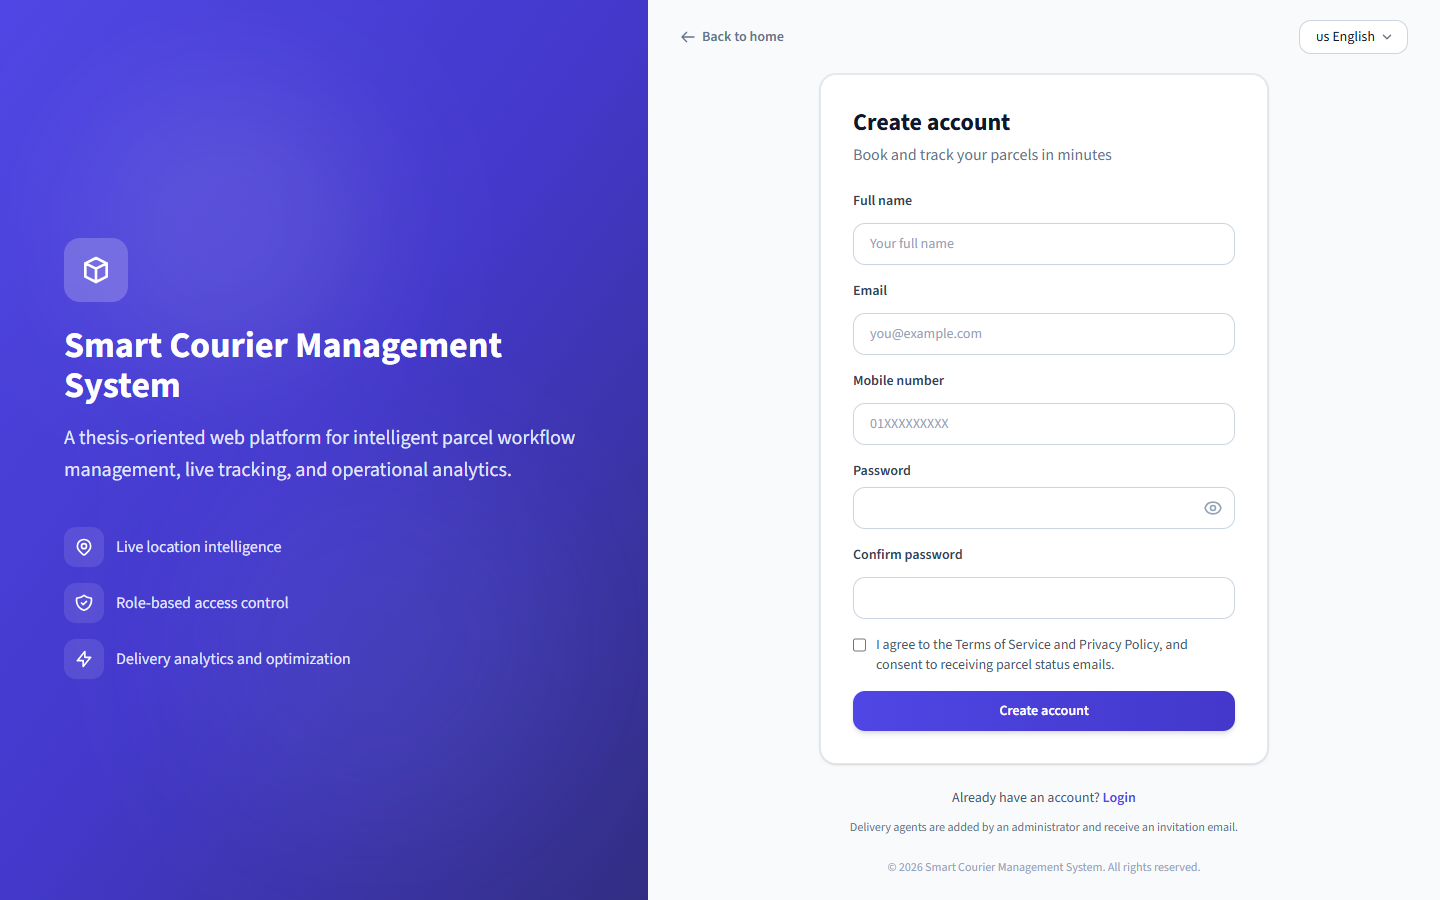
\includegraphics[width=0.85\textwidth]{figures/screenshots/register.png}
\caption{Customer registration page (running system)}
\label{fig:shot-register}
\end{figure}

\textbf{Login.} The login handler looks up the user with the hidden lockout fields. For unknown e-mails it still performs a bcrypt comparison against a dummy hash, so response time does not reveal whether an account exists. The lock is checked \emph{before} the password, so a correct guess during a lockout also fails. Five consecutive failures lock the account for 15 minutes. The account's active and verified states are revealed only after the password has been proven correct.

\textbf{Tokens and sessions.} A successful sign-in returns a JWT access token (HS256, issuer-checked, 15 minutes) containing the user id, role and \code{tokenVersion} (\code{tv}). It also sets a refresh cookie \code{scpms_rt}, a 384-bit random value, \code{HttpOnly}, \code{Secure} in production, \code{SameSite=Lax}, with path \code{/api/auth}. The frontend keeps the access token only in a JavaScript variable (\code{api.js}), never in \code{localStorage}. A timer refreshes the token one minute before expiry, and concurrent 401 responses share a single refresh request. Figure~\ref{fig:seq-session} shows the complete flow. When a refresh request arrives, the server handles the presented cookie as follows:
\begin{enumerate}
  \item It looks up the session by the hash of the cookie value. An unknown, expired or revoked session is refused (\code{NO_SESSION}).
  \item If the session was already rotated less than 30 seconds earlier, the request is treated as a harmless race between two browser tabs (\code{REFRESH_RACE}).
  \item If the session was rotated longer ago, the old cookie has been replayed, which indicates theft. Every session in the same rotation family is revoked (\code{TOKEN_REUSE}), so the legitimate user must also sign in again.
  \item Otherwise the session is marked as rotated, a new session with a fresh cookie is created in the same family, and a new access token is returned.
\end{enumerate}

\begin{figure}[htbp]
\centering
\resizebox{0.95\textwidth}{!}{% Sequence: sign-in, silent refresh with rotation and reuse detection
% (derived from auth.controller.js, session.service.js, frontend/src/api.js)
\begin{tikzpicture}[font=\scriptsize, >=Stealth]
\def\B{-12.2}
\seqhead{0}{b}{cCust}{Browser (React)}{\B}
\seqhead{6.0}{api}{cCore}{Express API}{\B}
\seqhead{11.0}{db}{cData}{Session collection}{\B}

% ---------------- sign in
\seqphase{-3.0}{12.2}{-0.75}{-3.85}{cCust}{1  SIGN IN}
\seqact{6.0}{-1.2}{-3.55}{cCore}
\seqmsg[cCust]{0}{5.91}{-1.35}{1}{POST /auth/login \{email, password, remember\}}
\seqnote{6.25}{-1.55}{lock check $\rightarrow$ bcrypt compare\\$\rightarrow$ active and verified}
\seqmsg[cData]{6.09}{11.0}{-2.65}{2}{store SHA-256(token), new family}
\seqret{5.91}{0}{-3.4}{access JWT (15 min, in memory)\\+ HttpOnly refresh cookie}

% ---------------- refresh
\seqphase{-3.0}{12.2}{-4.05}{-7.5}{cCore}{2  REFRESH}
\seqmsg[cCust]{0}{5.91}{-4.6}{3}{API requests with Authorization: Bearer}
\seqnote{0.3}{-4.95}{token near expiry, or 401 TOKEN\_EXPIRED}
\seqact{6.0}{-5.95}{-7.3}{cCore}
\seqmsg[cCust]{0}{5.91}{-6.1}{4}{POST /auth/refresh\\(cookie + X-Requested-With)}
\seqmsg[cData]{6.09}{11.0}{-6.6}{5}{mark old token rotated; store new hash}
\seqret{5.91}{0}{-7.15}{new access JWT + rotated cookie}

% ---------------- reuse detection
\seqphase{-3.0}{12.2}{-7.65}{-11.9}{cRed}{3  REUSE}
\pic at (-2.0,-8.05) {person=cRed};
\draw[cRed!60, line width=0.7pt, dash pattern=on 3pt off 2pt] (-2.0,-8.75) -- (-2.0,\B+0.3);
\seqact{6.0}{-8.25}{-11.45}{cRed}
\seqmsg[cRed]{-2.0}{5.91}{-8.4}{6}{attacker replays the old (already rotated) cookie}
\seqnote{6.25}{-8.6}{rotated more than 30 s ago\\$\Rightarrow$ reuse detected}
\seqmsg[cRed]{6.09}{11.0}{-9.65}{7}{revoke the whole token family}
\seqret[cRed]{5.91}{-2.0}{-10.3}{401 TOKEN\_REUSE}
\seqret[cRed]{5.91}{0}{-11.15}{legitimate session also ends: sign in again}
\end{tikzpicture}
}
\caption{Sequence diagram: sign-in, silent refresh with rotation, and reuse detection}
\label{fig:seq-session}
\end{figure}

The 30-second grace window handles a real case found during development: two browser tabs refreshing at the same moment present the same cookie, and the second request should not be treated as theft. The client retries once after a short delay when it receives \code{REFRESH_RACE}. Sessions last one day, or 30 days with ``Keep me signed in''. The two cookie-authenticated endpoints (\code{/auth/refresh} and \code{/auth/logout}) additionally require the header \cmd{X-Requested-With: XMLHttpRequest}, which a cross-site form cannot send.

\textbf{Password reset and revocation.} The forgot-password endpoint always returns the same message. When the account exists, it e-mails a single-use link whose token is stored hashed and expires after 30 minutes. Completing a reset increments \code{tokenVersion} and revokes all sessions. The same mechanism signs a user out everywhere when an administrator disables the account. \code{requireAuth} reloads the user on every request and rejects a token whose \code{tv} no longer matches.

\section{Authorisation}
\label{sec:impl-authz}

Authorisation is enforced on the server in two layers. The first layer is route guards: \code{requireAuth} verifies the token and loads the user, and \code{requireRoles(...)} admits only the listed roles. For example, booking is \code{requireRoles('customer')}, assignment and deletion are \code{requireRoles('admin')}, and location updates are \code{requireRoles('agent')}. The second layer is object-level checks in the controllers. \code{getParcel} returns a parcel only to its owner, its assigned agent or an administrator. \code{listParcels} adds a filter on \code{customer} or \code{agent} according to the role. \code{updateStatus} and \code{updateLocation} accept agents only for parcels assigned to them.

On the client, \code{ProtectedRoute}, \code{AdminRoute}, \code{DeliveryAgentRoute} and \code{CustomerRoute} redirect users away from pages for other roles. These guards improve usability but are not a security boundary, since the server repeats every check.

\section{Parcel Booking and Lifecycle}
\label{sec:impl-lifecycle}

\textbf{Booking.} Customers book from their dashboard (Figure~\ref{fig:shot-customer}). \code{createParcel} validates the addresses (1--300 characters), the enumerated fields, the COD amount (0--500{,}000, forced to 0 for prepaid parcels) and the notes ($\leq$500 characters). It then creates the parcel with an initial Pending history entry. The tracking code consists of ten characters drawn with \code{crypto.randomInt} from a 32-symbol alphabet that omits the easily confused characters 0, O, 1 and I. This gives $32^{10} = 2^{50}$ possible codes, which together with the rate limit on the public endpoint makes enumeration impractical. On the rare event of a duplicate code, creation is retried up to three times.

\begin{figure}[htbp]
\centering
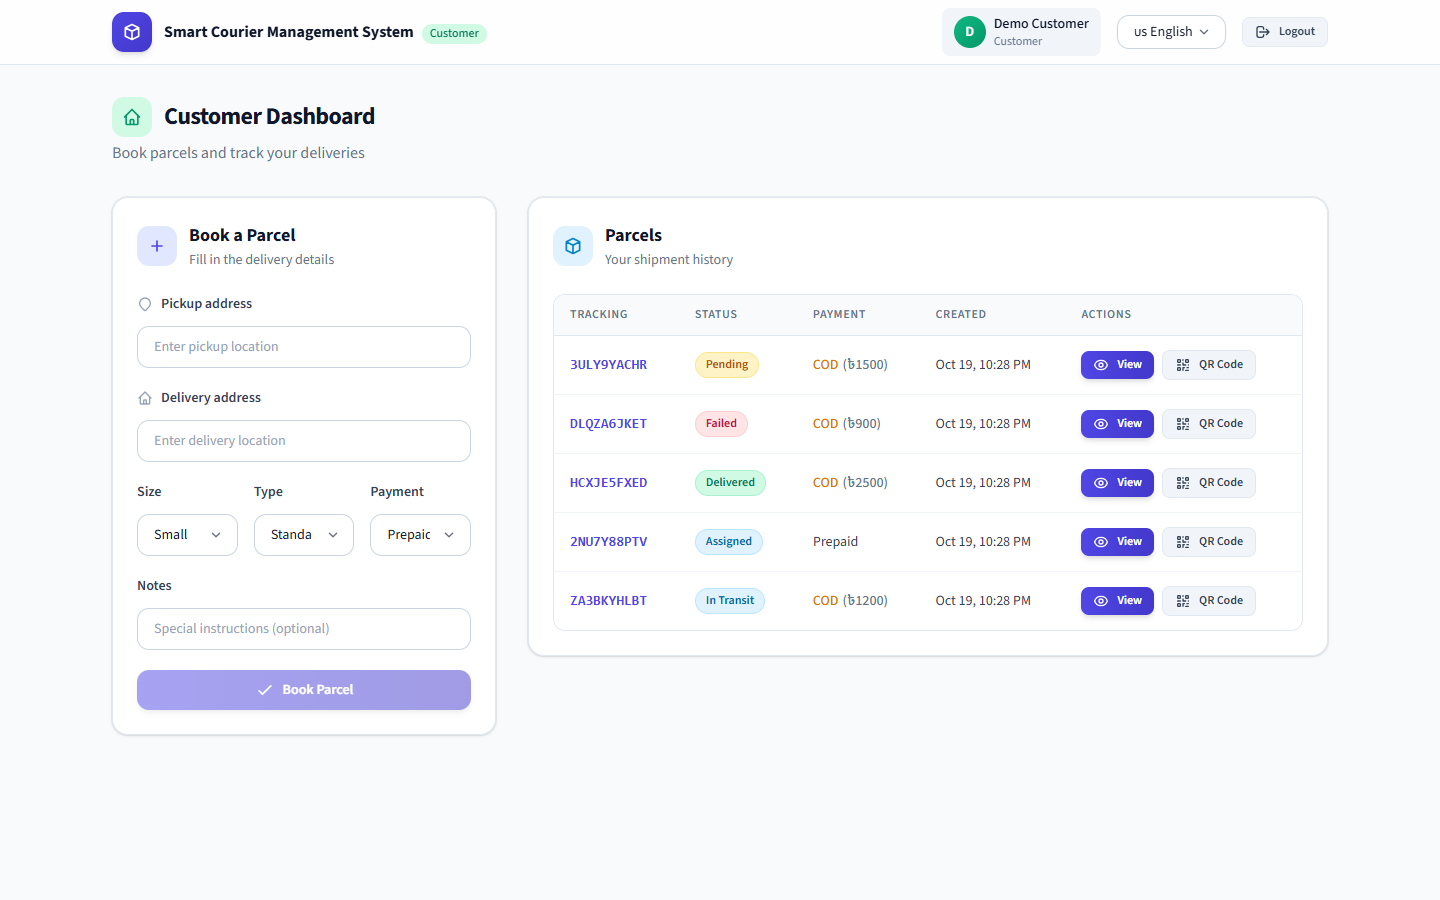
\includegraphics[width=0.9\textwidth]{figures/screenshots/customer-dashboard.png}
\caption{Customer dashboard with booking form and parcel list (running system, demonstration data)}
\label{fig:shot-customer}
\end{figure}

\textbf{Transitions.} All status changes go through one server-side rule, which encodes the state machine of Figure~\ref{fig:statemachine}. The rule applies its checks in a fixed order (Table~\ref{tab:transition-checks}). The first check that fails produces an explanatory error message, and the change is refused.

\begin{table}[htbp]
\centering
\caption{Order of checks applied to every requested status change}
\label{tab:transition-checks}
\small
\begin{tabularx}{\textwidth}{@{}p{0.6cm}LP{4.2cm}@{}}
\toprule
\textbf{No.} & \textbf{Check} & \textbf{Outcome} \\
\midrule
1 & The requested status equals the current status & Refused (``already in this state'') \\
2 & The parcel is Delivered or Failed & Refused for every role (final states are locked) \\
3 & The requester is an administrator & Allowed \\
4 & The parcel is not yet assigned to an agent (Pending) & Refused for agents \\
5 & The requested status is Failed & Allowed for the assigned agent \\
6 & The requested status lies before the current one, or is Pending or Assigned & Refused (agents only move forward) \\
7 & Any other forward move, including skipping states & Allowed \\
\bottomrule
\end{tabularx}
\end{table}

After a permitted change, the controller appends a history entry (status, time, actor and role) and saves the parcel. It then refreshes the agent's cached room list, pushes \code{parcel:update} to the watchers, and starts the status e-mail without waiting for it.

The agent's parcel page (Figure~\ref{fig:shot-agent-parcel}) shows the progress along the lifecycle, a status selector and controls for sending the current or a searched location.

\begin{figure}[htbp]
\centering
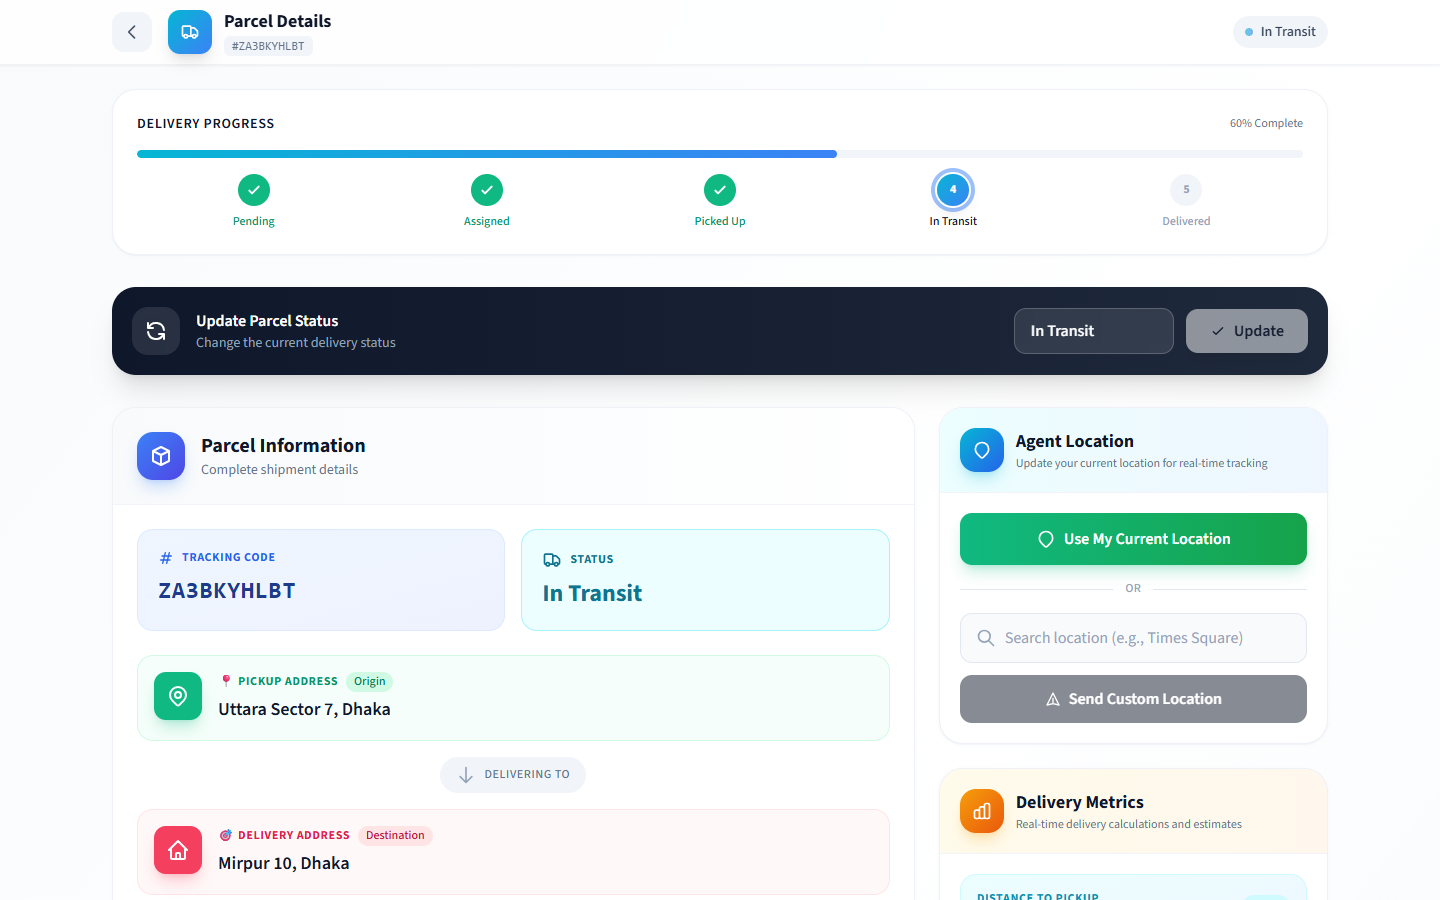
\includegraphics[width=0.9\textwidth]{figures/screenshots/agent-parcel-view.png}
\caption{Agent parcel page with lifecycle progress, status update and location controls (running system)}
\label{fig:shot-agent-parcel}
\end{figure}

\section{Real-Time Layer}
\label{sec:impl-realtime}

\code{services/socket.js} registers a Socket.IO middleware that reads \code{socket.handshake.auth.token}. If the token is valid and the user is active with a matching \code{tokenVersion}, it attaches \texttt{\{id, role\}} to the socket. Otherwise the socket stays anonymous. On connection, authenticated sockets join \code{user:<id>}, and administrators also join \code{role:admin}. The client reads the in-memory token at every (re)connection and reconnects after sign-in and sign-out, so the server always re-evaluates identity.

\code{services/realtime.js} provides \code{emitToParcel}, which sends to \code{role:admin}, \code{parcel:<id>}, the owning customer's room and the assigned agent's room, and \code{emitToAdmins}. Controllers emit only through these helpers. When an agent's browser sends a position, the server processes it in four steps:
\begin{enumerate}
  \item It discards the message unless the socket belongs to a signed-in agent and the agent identifier in the message is that agent's own identifier. This prevents anyone from spoofing another agent's position.
  \item It discards coordinates outside the valid latitude and longitude ranges.
  \item It stores the position in memory as the agent's last known location, with a timestamp.
  \item It forwards the position only to the administrators' room and to the rooms of the agent's active parcels (their watchers and owning customers).
\end{enumerate}
To avoid one database query per GPS update, the list of rooms for an agent's active parcels is cached for 15 seconds and refreshed whenever an assignment or status changes.

Administrators follow agents on the tracking page (Figure~\ref{fig:shot-tracking}). Selecting an agent loads that agent's parcels and sends \code{request:agent:location}. The server replies with the last known position and asks that agent's client, and only that client, for a fresh one.

\begin{figure}[htbp]
\centering
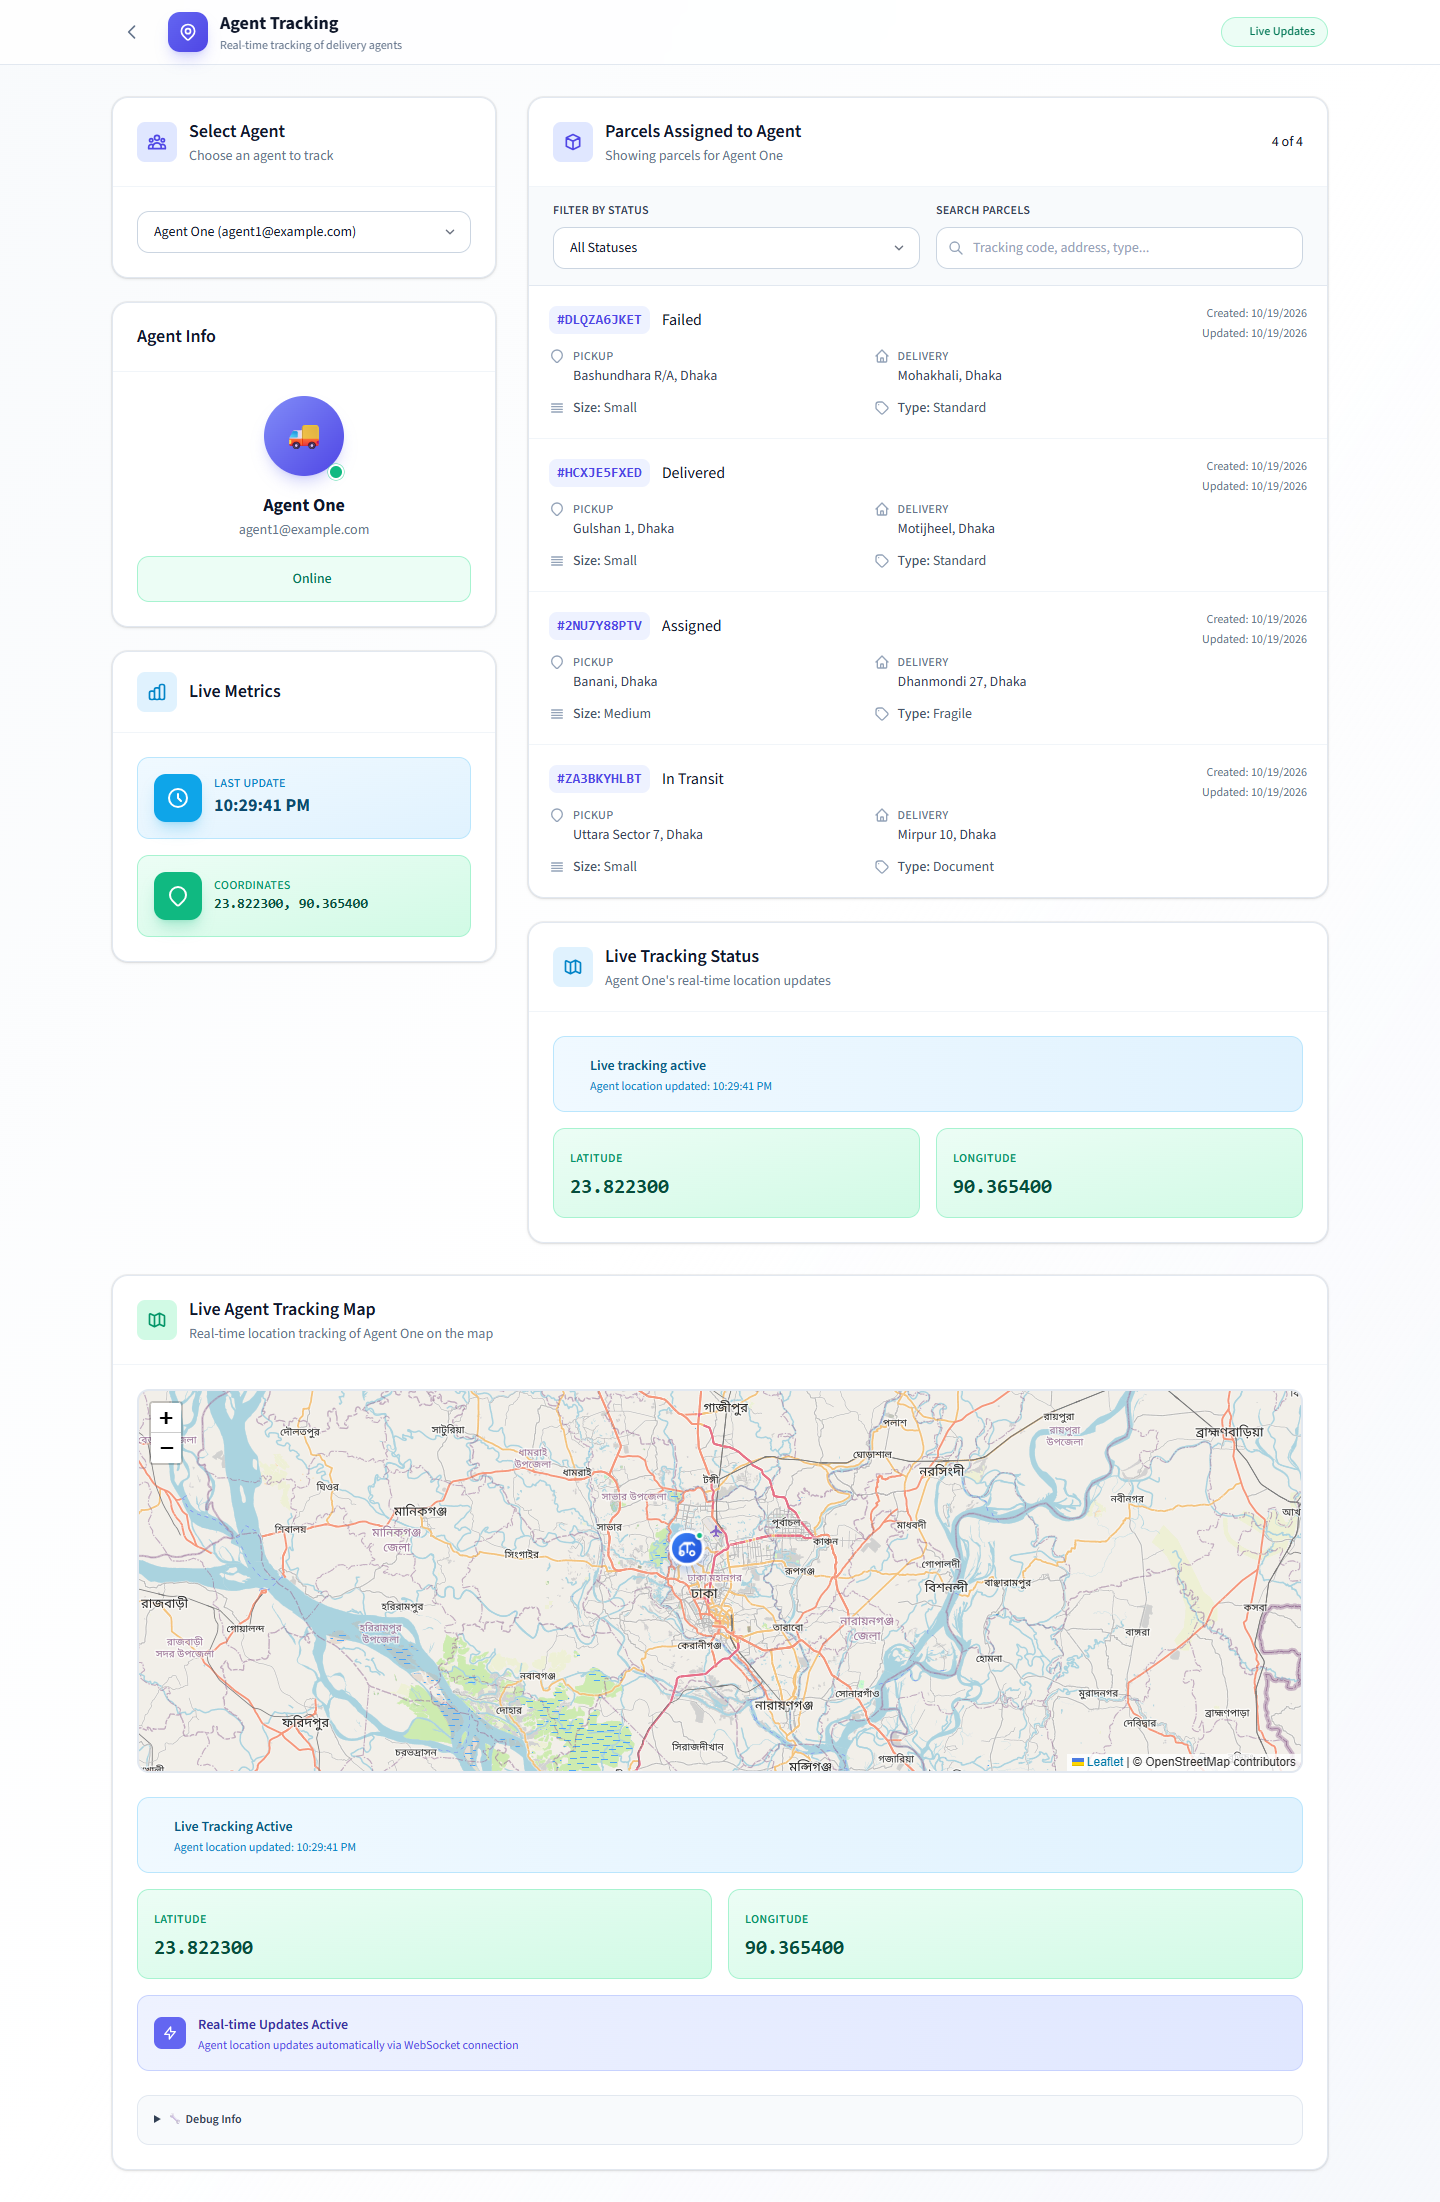
\includegraphics[width=0.78\textwidth]{figures/screenshots/admin-agent-tracking.png}
\caption{Administrator agent-tracking page receiving a live position from a connected agent (running system; position simulated)}
\label{fig:shot-tracking}
\end{figure}

\section{Location, Maps and Estimated Arrival}
\label{sec:impl-maps}

\textbf{Capturing location.} The agent dashboard calls \code{navigator.geolocation.watchPosition} with high accuracy. Each new position is throttled and skipped if unchanged, emitted on the socket, and posted through REST to every parcel that is In Transit. The agent's parcel page additionally sends the current position every 20 seconds, and allows a typed address to be geocoded and sent instead (for example when GPS is unavailable). The server accepts REST location updates only from the assigned agent and only for active parcels.

\textbf{Geocoding.} Addresses are free text. The backend route \code{/api/geocode/search} appends ``Bangladesh'', queries Photon biased towards Dhaka, and falls back to Nominatim with \code{countrycodes=bd} and an identifying \code{User-Agent} header. The route is rate-limited and caps the number of results at five, so it cannot be used for bulk lookups.

\textbf{Maps and routes.} Leaflet renders OSM tiles. leaflet-routing-machine requests a road route between the geocoded pickup and delivery points from the public OSRM demonstration server and draws it (Figures~\ref{fig:shot-public} and~\ref{fig:shot-customer-detail}). One page (\code{PublicTrack.jsx}, at \code{/track/:code}) uses the Google Maps JavaScript API instead. Its API key is not present in the repository's production environment file, so that page shows a map error unless the key is configured on the hosting platform. The Leaflet page \code{/track-parcel}, linked from status e-mails, does not depend on Google.

\begin{figure}[htbp]
\centering
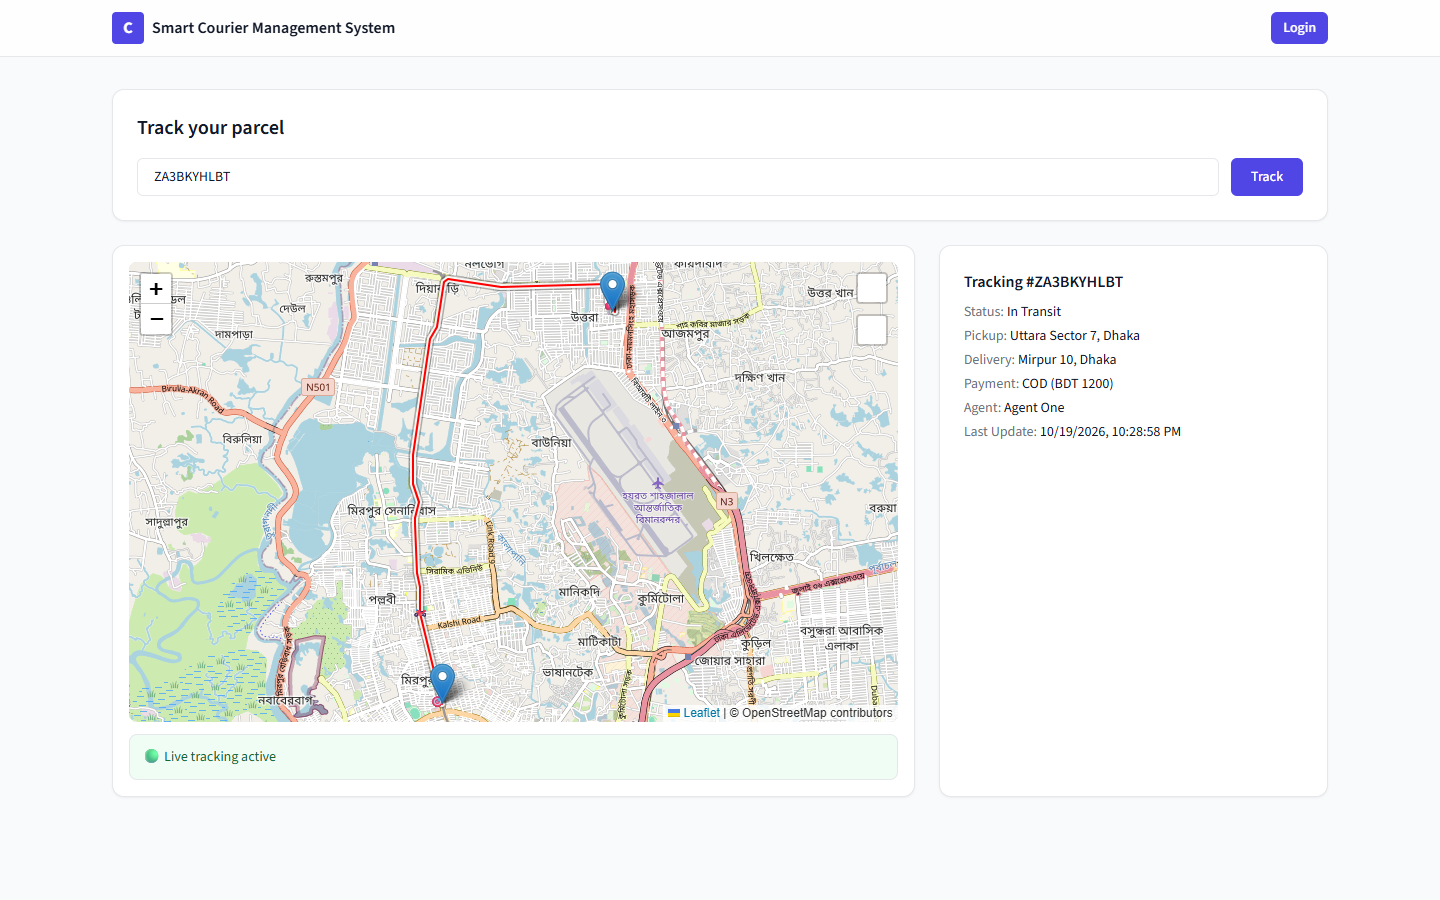
\includegraphics[width=0.9\textwidth]{figures/screenshots/public-tracking.png}
\caption{Public tracking by code with OSM map and OSRM route; no customer data is shown (running system)}
\label{fig:shot-public}
\end{figure}

\textbf{Estimated arrival.} The customer parcel page computes the straight-line (haversine) distance from the agent's latest position to the geocoded delivery point. It divides this distance by the agent's observed speed, or by 25\,km/h when no speed is known, to display an ETA (Figure~\ref{fig:shot-customer-detail}). This is a simple heuristic, not a road-network or traffic-aware prediction, and it is presented as such in this report. The server stores \code{etaMinutes} only when a client supplies it.

\begin{figure}[htbp]
\centering
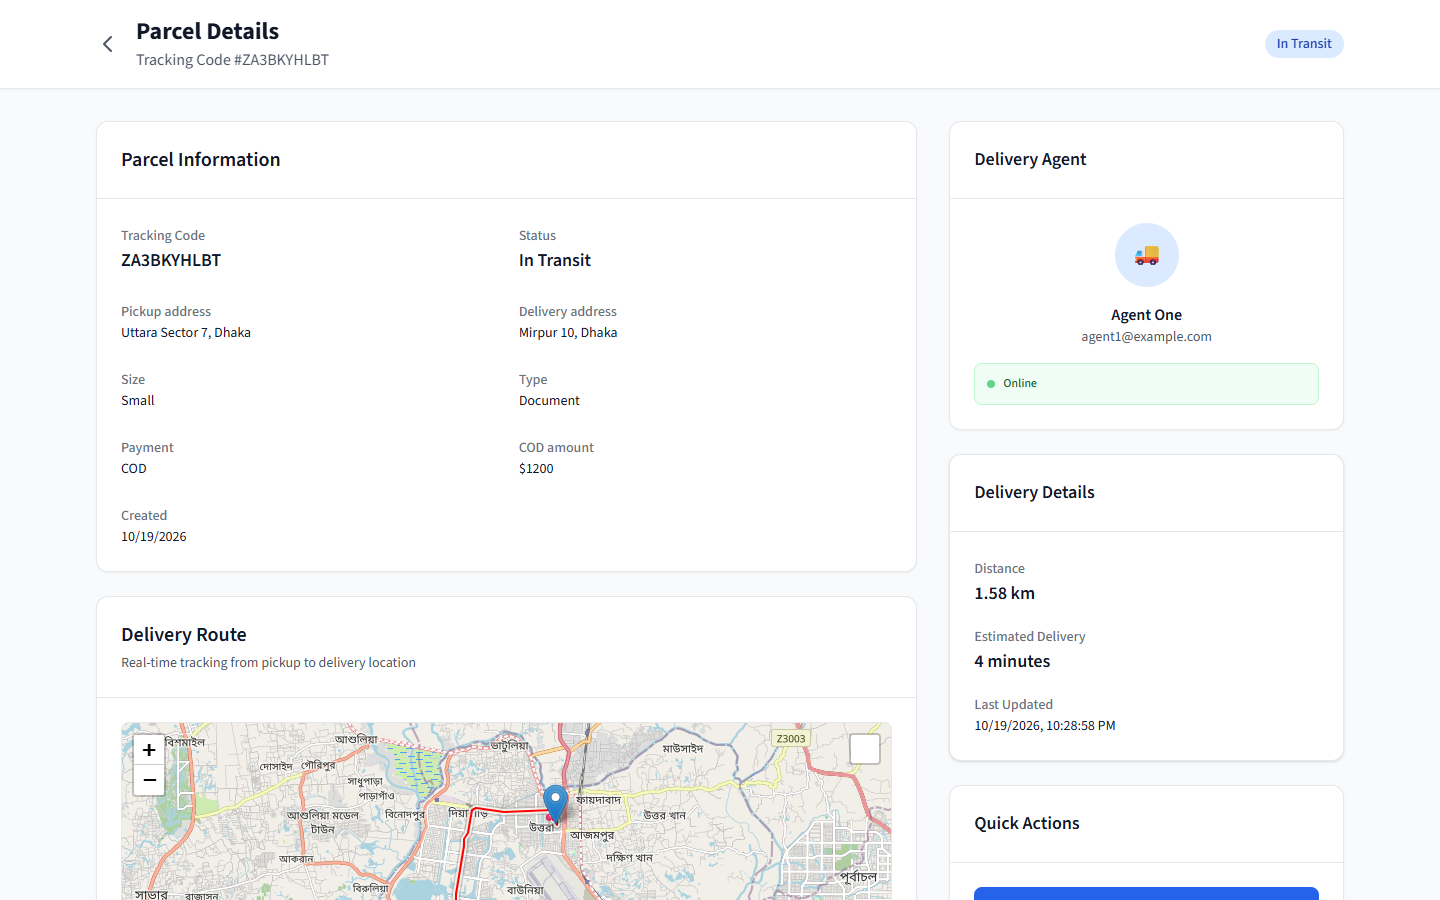
\includegraphics[width=0.9\textwidth]{figures/screenshots/customer-parcel-detail.png}
\caption{Customer parcel page with agent card, distance and heuristic ETA (running system). The COD amount is shown with a ``\$'' sign, a currency-symbol defect recorded in Chapter~\ref{chap:results}}
\label{fig:shot-customer-detail}
\end{figure}

\section{QR-Assisted Pickup}
\label{sec:impl-qr}

For each parcel the customer can open a QR page (Figure~\ref{fig:shot-qr}). The page encodes the URL \code{<origin>/customer/parcel/qr/<parcelId>} with the \code{qrcode} library at error-correction level~M, and offers a print button. The agent opens ``Pickup Scan'' from the dashboard. The scanner uses the browser's native \code{BarcodeDetector} when available, sampling the rear camera every 250\,ms, and otherwise falls back to ZXing. It extracts the parcel id from the scanned URL and opens the confirmation page (Figure~\ref{fig:shot-pickup}). Confirming sends \texttt{\{status: "Picked Up"\}}. If the camera cannot be used, the agent can paste the link or the parcel id.

\begin{figure}[htbp]
\centering
\begin{subfigure}[t]{0.49\textwidth}
  \centering
  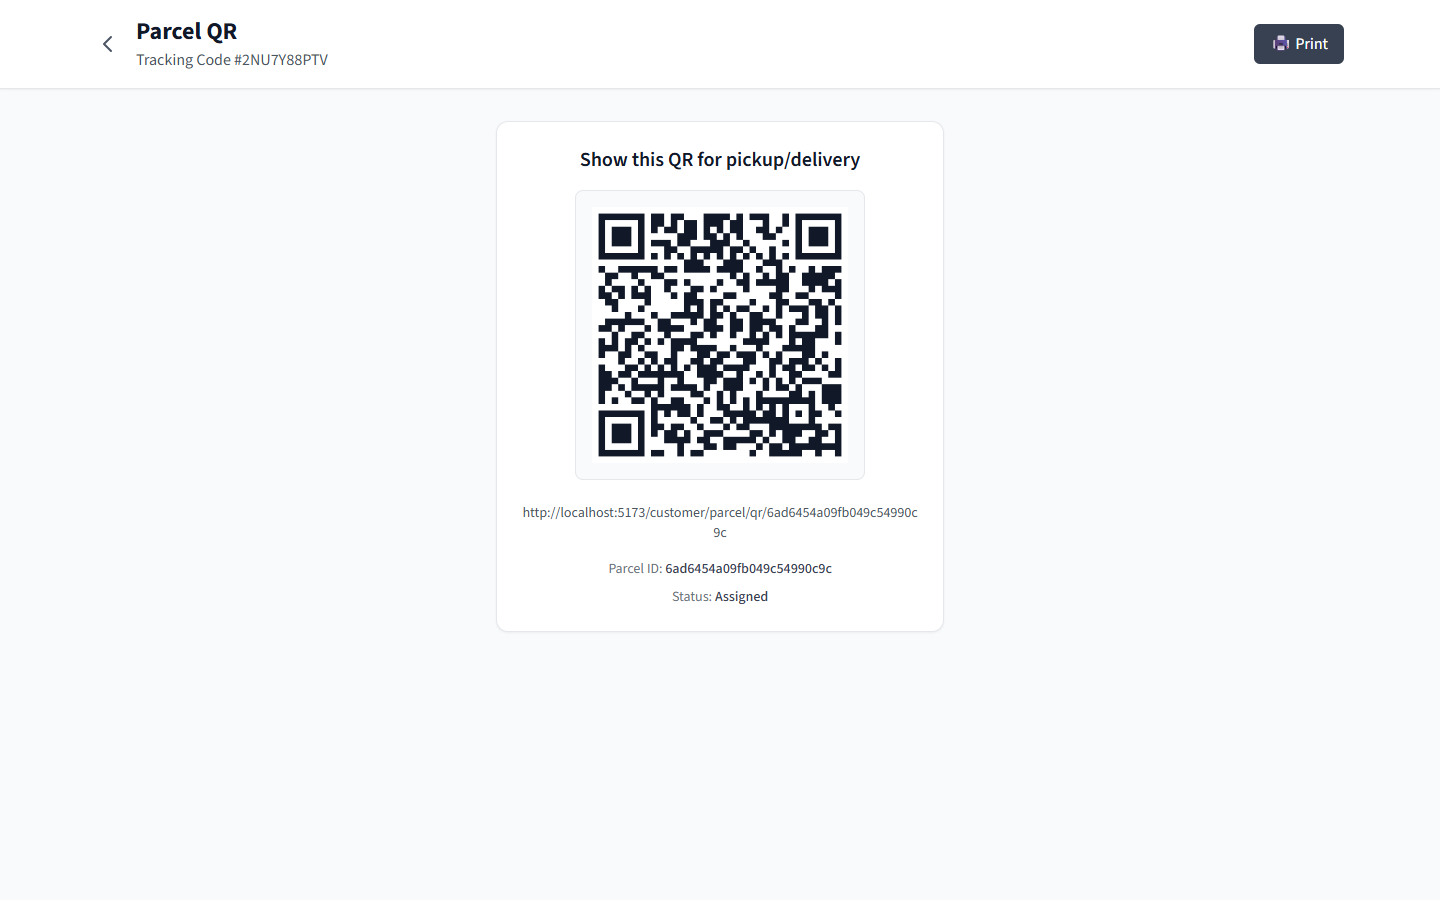
\includegraphics[width=\textwidth]{figures/screenshots/customer-qr.png}
  \caption{Customer's parcel QR page}
  \label{fig:shot-qr}
\end{subfigure}\hfill
\begin{subfigure}[t]{0.49\textwidth}
  \centering
  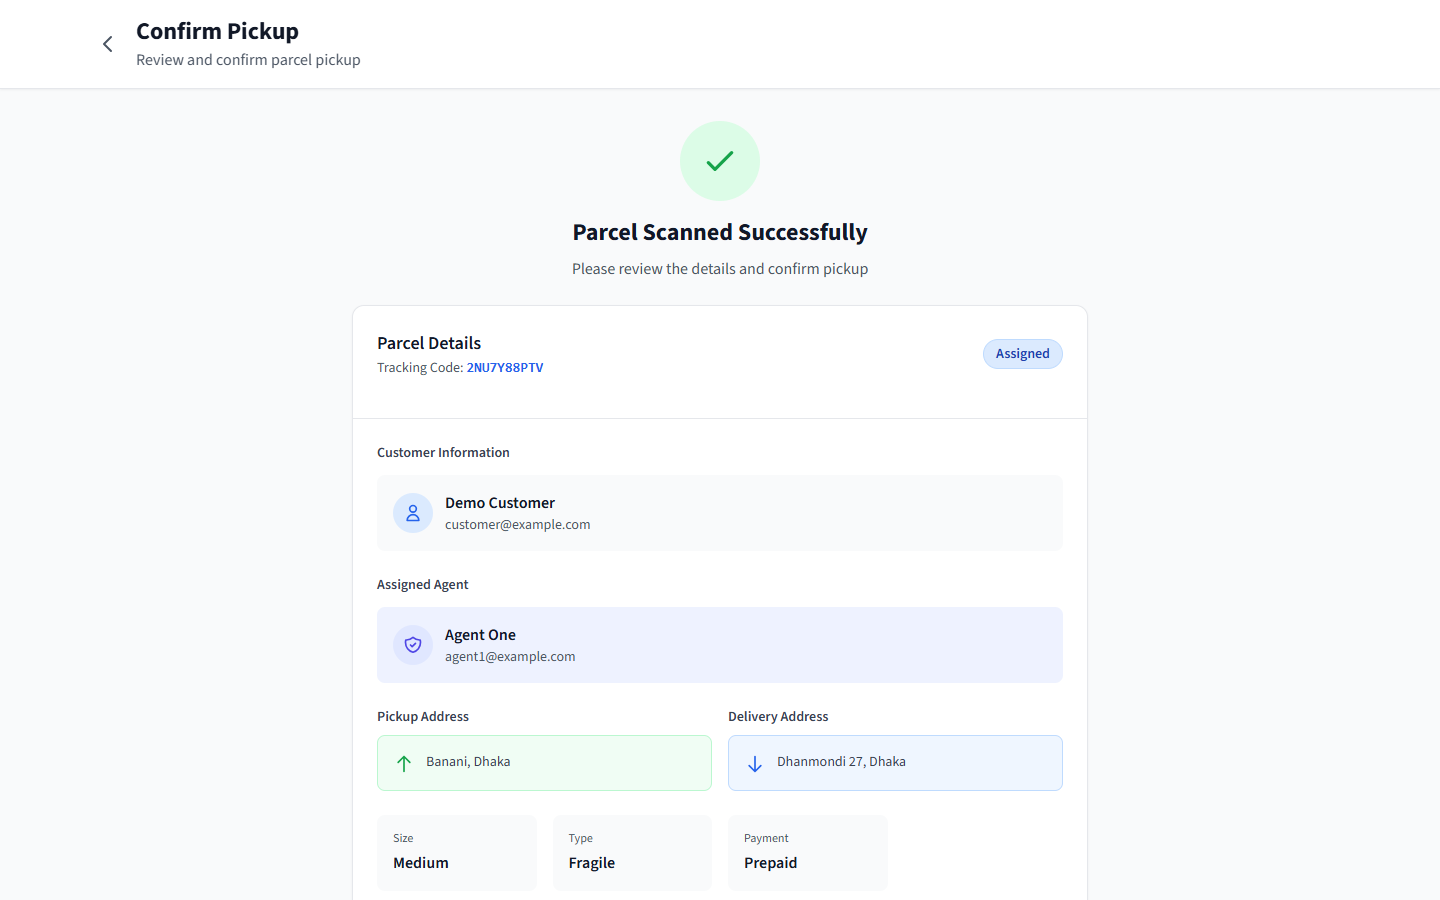
\includegraphics[width=\textwidth]{figures/screenshots/agent-pickup-confirm.png}
  \caption{Agent's pickup confirmation page}
  \label{fig:shot-pickup}
\end{subfigure}
\caption{QR-assisted pickup (running system). The confirmation page is normally reached by scanning; for the screenshot it was opened directly by URL}
\label{fig:shot-qrflow}
\end{figure}

It is important to state precisely what the QR step achieves. It \emph{identifies} the parcel quickly and reduces the chance that an agent confirms the wrong parcel. It is \emph{not} a cryptographic proof of handover. The QR content is the parcel's database identifier, and the manual fallback accepts the same identifier. The security guarantee comes from the server, which accepts the Picked Up transition only from the agent assigned to that parcel. The QR page's heading mentions ``pickup/delivery'', but scanning is implemented only for pickup. Earlier project documents that describe QR verification at delivery, or OTP delivery confirmation, describe features that are not present: the OTP interface was removed during the security review because it had no backend.

\section{Notifications}
\label{sec:impl-notify}

\code{utils/mailer.js} builds HTML e-mails with a shared layout and escapes all user-supplied text to prevent HTML injection. Four message types exist: the verification code, the password-reset link, the agent invitation (72-hour link) and the status-change notification. The status notification links to the public tracking page. It is sent asynchronously after the database update, and failures are only logged, so an unavailable SMTP server cannot delay or fail a status change. In production, an unconfigured mailer makes the verification, reset and invitation operations return 503. If an invitation cannot be e-mailed, the administrator is shown the link to share by another channel.

\section{Analytics, Export and User Management}
\label{sec:impl-analytics}

The administrator dashboard (Figure~\ref{fig:shot-admin}) shows three indicators computed by \code{dashboardMetrics}: bookings created since local midnight, the number of parcels in the Failed state, and the sum of COD amounts of delivered COD parcels (a MongoDB aggregation). The indicators refresh when \code{parcel:created} or \code{parcel:update} events arrive. The bookings table supports text search by tracking code or status and per-row assignment, and the assignment control locks once a parcel is past Assigned. The CSV export streams one row per parcel (tracking code, status, payment type, COD amount, creation time) with proper quoting. The PDF export writes the same fields as a simple list with PDFKit. The users panel lists all accounts with their state (active, unverified or invitation pending, disabled) and lets the administrator add agents, resend invitations and disable or re-enable accounts.

\begin{figure}[htbp]
\centering
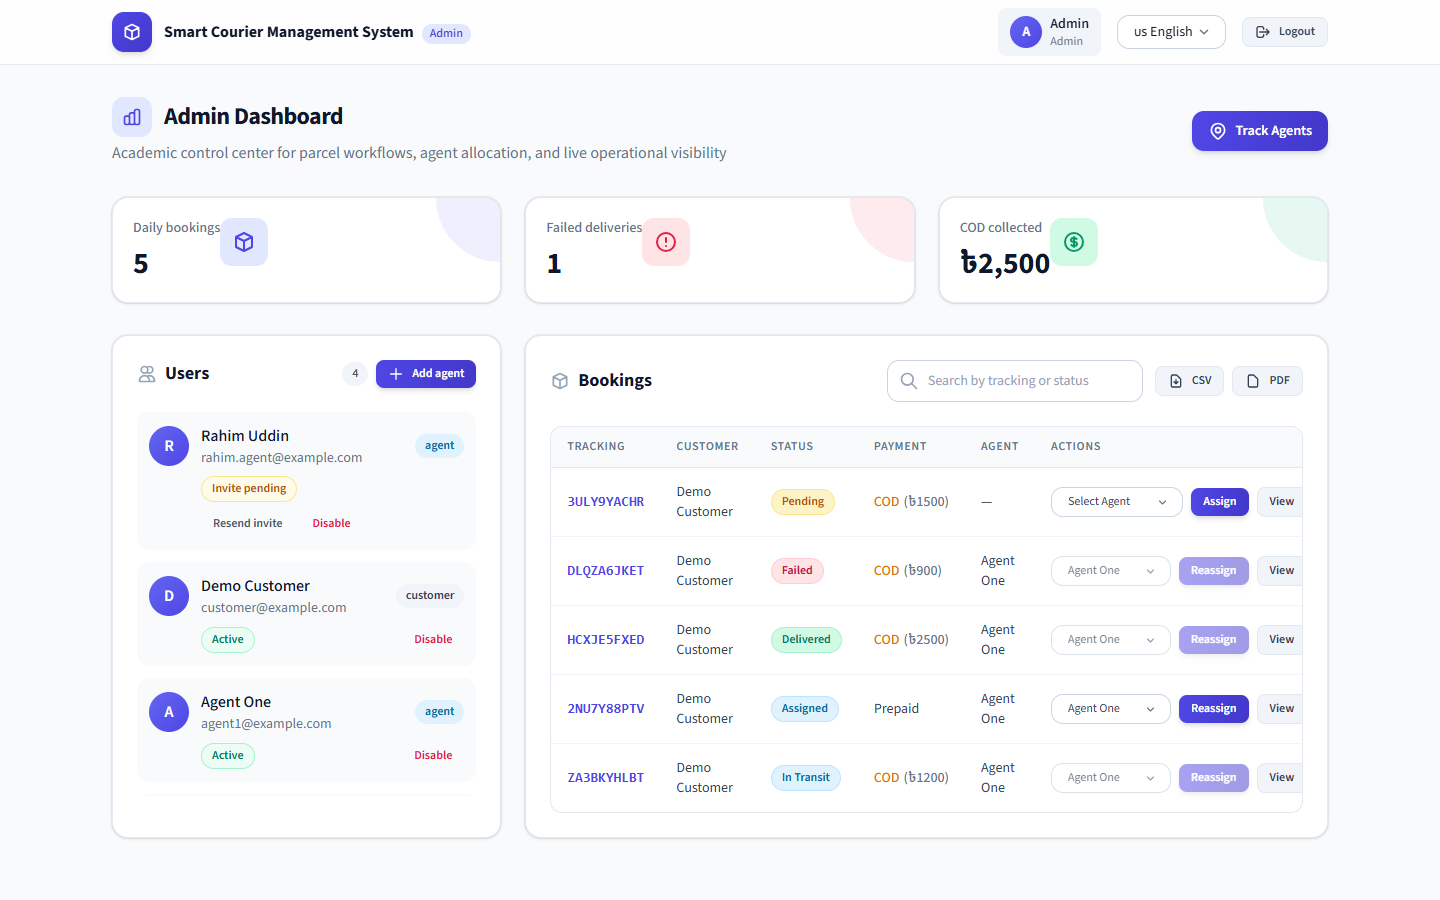
\includegraphics[width=0.95\textwidth]{figures/screenshots/admin-dashboard.png}
\caption{Administrator dashboard: indicators, user management, bookings with assignment and CSV/PDF export (running system, demonstration data)}
\label{fig:shot-admin}
\end{figure}

The analytics are deliberately basic. The system does not compute success rates over time, revenue trends, monthly reports, heat maps or delay risk, although some early documents listed them. They remain future work.

\section{Frontend Implementation and Internationalisation}
\label{sec:impl-frontend}

The frontend is a React single-page application. \code{App.jsx} defines public routes (landing, tracking, login, registration, verification, password reset), guest-only routes and role-guarded route groups. \code{AuthContext} restores the session on page load by calling the refresh endpoint (the access token is not persisted), schedules the next refresh and reconnects the shared socket when identity changes. \code{api.js} attaches the bearer token, retries once after a successful refresh on token errors, and converts server errors into an \code{ApiError} carrying the machine-readable code (for example \code{EMAIL_NOT_VERIFIED}). The UI uses these codes to show helpful messages.

\begin{figure}[htbp]
\centering
\begin{subfigure}[t]{0.49\textwidth}
  \centering
  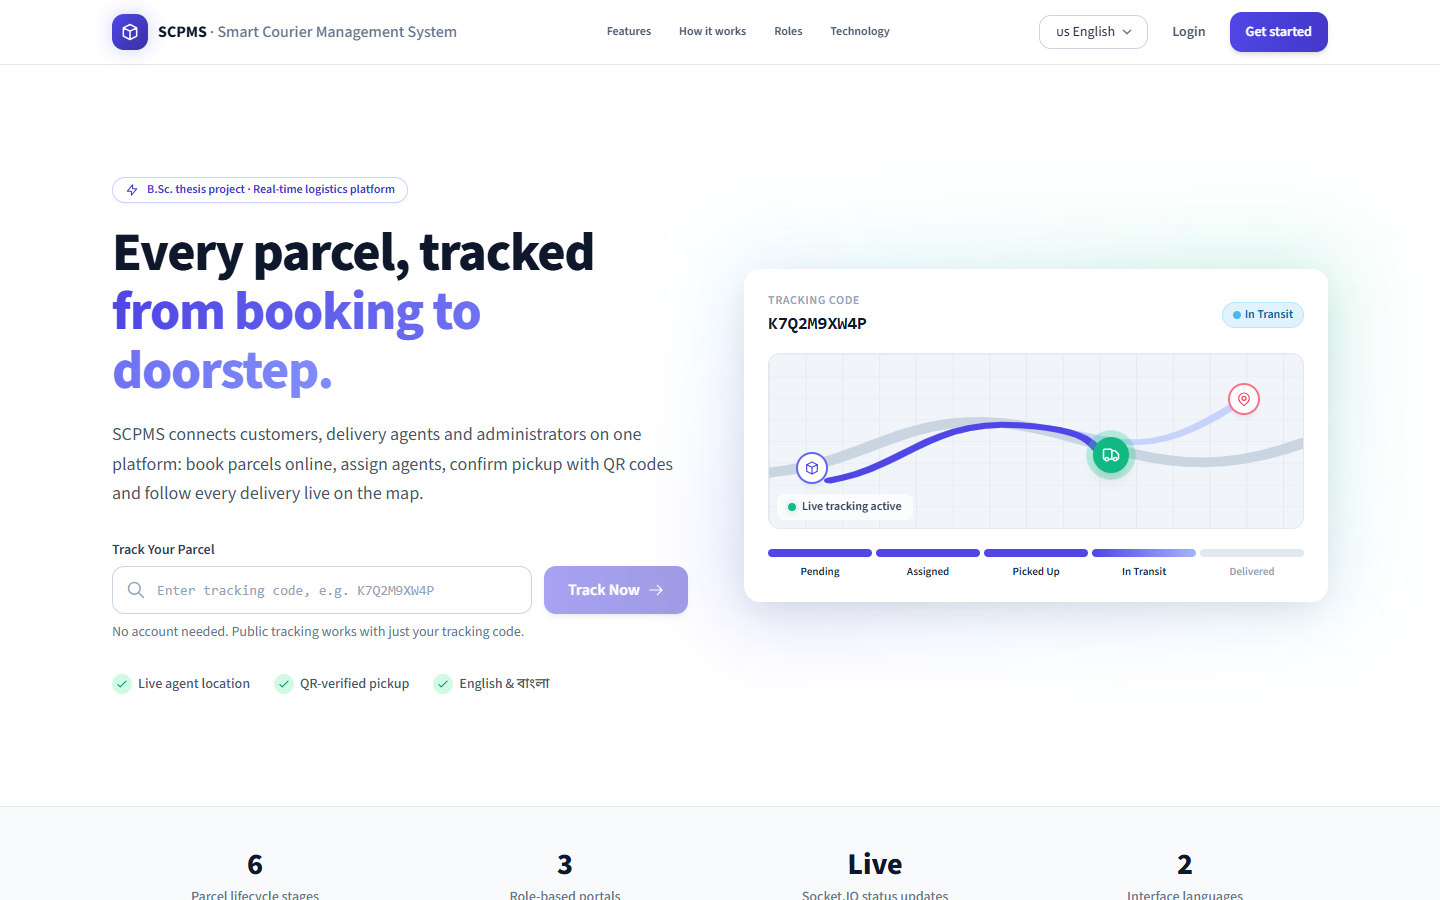
\includegraphics[width=\textwidth]{figures/screenshots/landing.png}
  \caption{English}
\end{subfigure}\hfill
\begin{subfigure}[t]{0.49\textwidth}
  \centering
  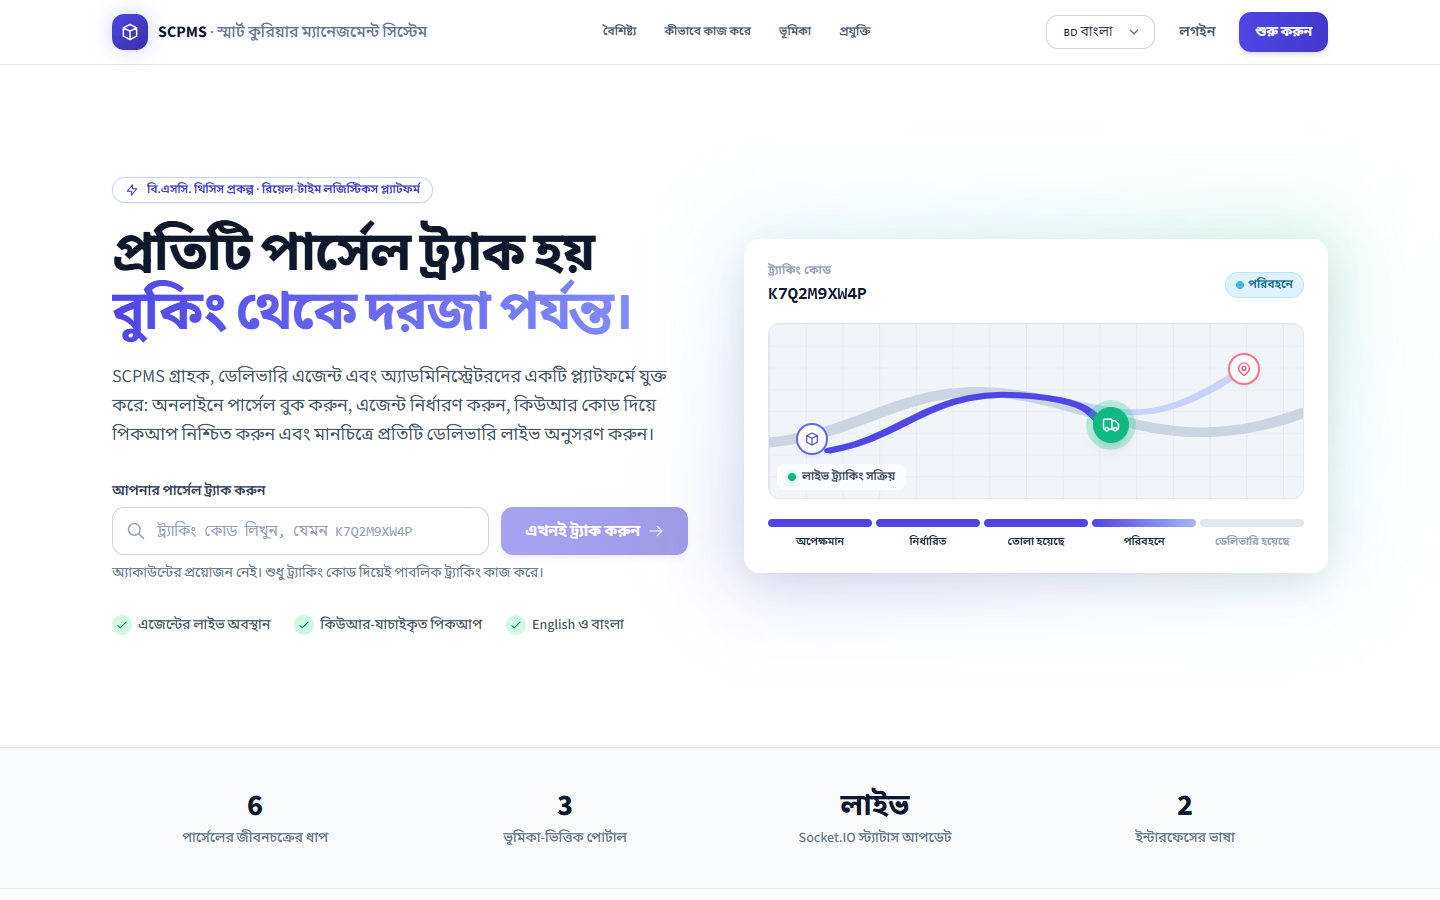
\includegraphics[width=\textwidth]{figures/screenshots/landing-bn.png}
  \caption{Bangla}
\end{subfigure}
\caption{Landing page with public tracking entry in both interface languages (running system)}
\label{fig:shot-landing}
\end{figure}

\code{LanguageContext} stores the chosen language in \code{localStorage}, and each component reads its strings from \code{translations/en.js} or \code{bn.js}, which hold about 320 entries each. Figure~\ref{fig:shot-landing} shows the landing page in both languages. The agent dashboard (Figure~\ref{fig:shot-agent}) summarises the agent's parcels, shows the socket connection state and a live OSM map of the agent's own position, and links to the pickup scanner.

\begin{figure}[htbp]
\centering
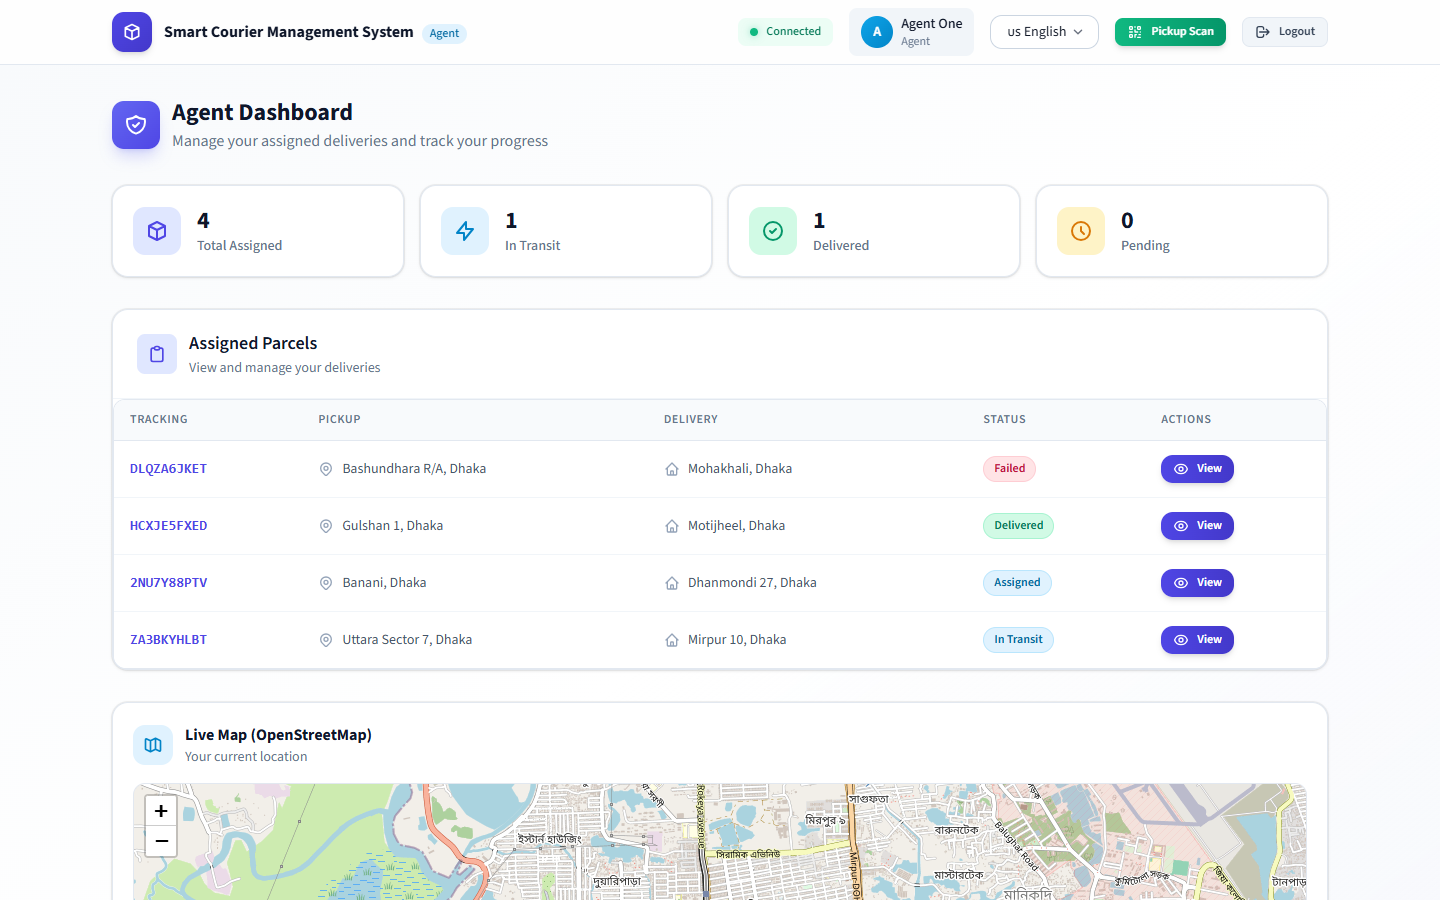
\includegraphics[width=0.9\textwidth]{figures/screenshots/agent-dashboard.png}
\caption{Delivery-agent dashboard (running system, demonstration data)}
\label{fig:shot-agent}
\end{figure}

\section{Validation, Error Handling and Hardening}
\label{sec:impl-hardening}

Input is validated at three levels. First, \code{middleware/sanitize.js} recursively removes every key that begins with \code{$} or contains \code{.} from the body, query string and route parameters, so values such as \texttt{\{"\$ne": null\}} can never reach MongoDB as operators \cite{ron2016nosql}. Second, controllers check types and ranges explicitly: identifiers with \code{isObjectId}, coordinates with \code{isValidLatLng}, strings with length limits, and enumerations against the shared constants. Third, Mongoose schema constraints act as a final safeguard. Mongoose's \code{strictQuery} option discards unknown query fields.

Rate limits are applied per endpoint: login (20 per 15 minutes), registration (10 per hour), code verification and password reset (20 per 15 minutes), e-mail-sending endpoints (5 per 15 minutes), refresh (120), public tracking (120) and geocoding (300 per 15 minutes), on top of the global limit. The number of trusted proxy hops is configurable (\code{TRUST_PROXY_HOPS}), so that the limiter sees real client addresses behind the hosting proxies. The frontend hosting configuration adds \code{X-Frame-Options}, \code{X-Content-Type-Options}, \code{Referrer-Policy}, HSTS and a \code{Permissions-Policy} that allows camera and geolocation only for the site itself.

\section{Deployment and Execution}
\label{sec:impl-deploy}

Figure~\ref{fig:deployment} shows the deployment that the repository is configured for. \code{backend/render.yaml} defines a Render web service with a \code{/health} check, \code{NODE_ENV=production}, two trusted proxy hops, a generated \code{JWT_SECRET}, and placeholders for the database URI, allowed origin, application URL and SMTP credentials. \code{frontend/vercel.json} and \code{netlify.toml} serve the built SPA, rewrite \code{/api/*} to the Render service and set security headers. \code{frontend/.env.production} sets \code{VITE_API_BASE=/api} and the socket URL. Whether this deployment is currently running was not verified as part of this work.

\begin{figure}[htbp]
\centering
\resizebox{\textwidth}{!}{% Deployment view (derived from backend/render.yaml, frontend/vercel.json, netlify.toml,
% frontend/.env.production). Whether the deployment is currently live was not verified.
\begin{tikzpicture}[font=\scriptsize, >=Stealth,
  box/.style={card=#1, minimum width=3.8cm, minimum height=1.9cm, align=center, text width=3.5cm},
  svc/.style={card=#1, minimum width=2.9cm, minimum height=1.5cm, align=center, text width=2.6cm}]

% ---------- zones
\node[panel=cCust, minimum width=4.6cm, minimum height=6.4cm] at (0,-1.15) {};
\node[tag=cCust] at (0,1.75) {CLIENT DEVICES};
\node[panel=cExt, minimum width=4.6cm, minimum height=3.1cm] at (5.8,0.5) {};
\node[tag=cExt] at (5.8,1.75) {STATIC HOSTING / EDGE};
\node[panel=cCore, minimum width=4.6cm, minimum height=3.1cm] at (11.6,0.5) {};
\node[tag=cCore] at (11.6,1.75) {APPLICATION TIER};
\node[panel=cData, minimum width=10.4cm, minimum height=2.6cm] at (8.7,-3.05) {};
\node[tag=cData, anchor=west] at (3.65,-4.35) {DATA AND THIRD-PARTY SERVICES};

% ---------- main nodes (icons sit in the reserved top area of each card)
\node[box=cCust] (browser) at (0,0.25) {\iconspace[8mm]\textbf{Browser}\\desktop or phone};
\pic at (-0.5,0.78) {browser=cCust}; \pic at (0.6,0.78) {phone=cCust};
\node[box=cExt] (cdn) at (5.8,0.25) {\iconspace[8mm]\textbf{Vercel / Netlify}\\SPA files, \code{/api/*} rewrite,\\security headers};
\node[cloud, cloud puffs=10, aspect=2, draw=cExt, fill=cExt!20, line width=0.8pt, minimum width=1.2cm, minimum height=0.65cm] at (5.8,0.85) {};
\node[box=cCore] (render) at (11.6,0.25) {\iconspace[8mm]\textbf{Render web service}\\Express + Socket.IO,\\health check \code{/health}};
\pic at (11.6,0.82) {server=cCore};

\node[svc=cData] (db) at (5.6,-3.25) {\iconspace[7mm]\textbf{MongoDB}\\\code{MONGODB_URI}};
\pic at (5.6,-2.88) {db=cData};
\node[svc=cExt] (smtp) at (8.7,-3.25) {\iconspace[7mm]\textbf{SMTP}\\Gmail (app password)};
\pic at (8.7,-2.86) {mail=cExt};
\node[svc=cExt] (geo) at (11.8,-3.25) {\iconspace[7mm]\textbf{Geocoding}\\Photon / Nominatim};
\pic at (11.8,-2.82) {pin=cRed};
\node[box=cExt, minimum height=1.6cm] (maps) at (0,-3.25) {\iconspace[7mm]\textbf{Map services}\\OSM tiles, OSRM demo, Google Maps JS};
\pic at (0,-2.82) {mapicon=cExt};

% ---------- connections
\draw[flow=cCust] (browser.east) -- node[elabel, above=2pt]{HTTPS: pages\\and \code{/api}} (cdn.west);
\draw[flow=cExt] (cdn.east) -- node[elabel, above=2pt]{proxied\\\code{/api}} (render.west);
\draw[rtflow] ($(browser.north east)+(-0.5,0.25)$) -- ++(0,1.25) -| node[pos=0.25, above, font=\scriptsize\bfseries, text=cSock]{WebSocket connection directly to the backend (\code{VITE_SOCKET_URL})} ($(render.north east)+(-0.25,0.25)$);
\draw[bflow=cData] ($(render.south)+(-1.2,0)$) -- (db.north east);
\draw[flow=cExt] ($(render.south)+(-0.3,0)$) -- (smtp.north);
\draw[bflow=cExt] ($(render.south)+(0.3,0)$) -- (geo.north);
\draw[bflow=cExt] (browser.south) -- (maps.north);

\node[font=\tiny, text=cExt, anchor=north west] at (-2.3,-4.75) {Configuration as defined in the project files; whether this deployment is currently live was not verified.};
\end{tikzpicture}
}
\caption{Deployment view as configured in the repository}
\label{fig:deployment}
\end{figure}

For local execution, the dependencies of both packages are installed from the repository root. A seed script creates the first administrator and agent; in production, their passwords must be supplied through environment variables. A single development script then starts the API on port 5000 and the web client on port 5173.

\section{Implementation Challenges}
\label{sec:challenges}

\begin{itemize}
  \item \textbf{Securing real-time channels.} The first version trusted the \code{agentId} sent by any socket and broadcast all agent positions to every client, so locations could be spoofed and leaked. Authenticating sockets with the access token and scoping every event to rooms solved both problems. It required the room cache to keep database load low during continuous GPS updates.
  \item \textbf{Cookies across hosting providers.} With the frontend and API on different domains, browsers that block third-party cookies dropped the refresh cookie. Routing \code{/api} through the frontend host made the cookie first-party.
  \item \textbf{Configuration loaded too late.} Some modules read \code{process.env} when imported, before \code{.env} had been loaded, so local SMTP and JWT settings were silently ignored. Loading \code{dotenv} as the first import fixed this.
  \item \textbf{Concurrent refreshes.} Rotating refresh tokens broke sessions when two tabs refreshed together. The 30-second grace window and a single client retry handle this race without weakening reuse detection.
  \item \textbf{Free map services.} Geocoding of informal Bangladeshi addresses is sometimes imprecise, and public routing and geocoding services impose rate limits. A backend proxy with Bangladesh bias and a Photon-to-Nominatim fallback mitigates, but does not remove, this dependency.
  \item \textbf{Camera access.} Browser camera access requires HTTPS and user permission, and \code{BarcodeDetector} is not available everywhere. The ZXing fallback and manual entry keep pickup possible.
\end{itemize}

\section{Summary}

This chapter turned the problem and the literature into 21 functional and seven non-functional requirements, presented the design that meets them and described its implementation. The design consists of a layered single-process backend with a three-collection data model, a server-enforced six-state lifecycle with an embedded audit trail, room-scoped real-time events, and a layered security design mapped to the OWASP Top~10. The implementation realises this design in about 11,000 lines of JavaScript. The backend enforces authentication, authorisation and the parcel lifecycle in one place and delivers real-time events only to authorised rooms. The frontend provides three role-specific interfaces, public tracking, maps, QR-assisted pickup and a bilingual interface. The screenshots confirm that these features run end to end. Chapter~\ref{chap:results} evaluates the implementation against the requirements.
